\section{Introducción}
%%%%%%%%%%%%%%%%%%%%%%%%%%%%%%%%55%%%%%%%%%%%%%%%%%%%%%%%%%%%%%%%%%%%%%%%%%%%%%%%%%%%%%%%%%%%%%%%%%%%%%%%%%%%%%%%%%%%%%%%%%%%%%%%%%
% requerimientos,Hacer como una sinopsis.
%%%%%%%%%%%%%%%%%%%%%%%%%%%%%%%%%%%%%%%%%%%%%%%%%%%%%%%%%%%%%%%%%%%%%%%%%%%%%%%%%%%%%%%%%%%%%%%%%%%%%%%%%%%%%%%%%%%%%%%%%%%%%%%%%%%

En este documento se describen las tareas realizadas en el marco del proyecto de fin de carrera ``Análisis de Video en Biomecánica'' realizado en la Facultad de Ingeniería, Udelar. En este capítulo, se realiza una introducción al problema planteado y en función de esto se plantea el objetivo para el proyecto y una breve revisión del estado del arte para los sistemas de estas características.

\vspace{5 mm}

Especialistas de distintos ámbitos académicos o profesionales se encuentran habitualmente en la necesidad de realizar estudios del movimiento del cuerpo humano. Esta tarea implica registrar la posición de miembros o articulaciones en el espacio y su correspondiente evolución en el tiempo.

Algunos ejemplos correspondientes a distintas áreas que ilustran estas necesidades son:

\begin{itemize}
\item A \emph{nivel asistencial}, en el área de \emph{fisioterapia}. Para realizar un seguimiento de la evolución de un paciente resulta importante en muchos casos conocer en detalle el movimiento, posición, etc. de la articulación o miembro afectado para llevar un control del mismo durante la rehabilitación y así poder determinar con mayor exactitud el estado del paciente.
\item \emph{Investigación académica en biomecánica}. Diversos proyectos se llevan a cabo en las universidades sobre esta temática, por ejemplo, en la Facultad de Ingeniería de la Udelar  se realizó el estudio comparativo de la patada delfín y la patada “crawl” respecto al nado de los peces por ondulación, tratando de explicar cómo la misma puede ser propulsiva. Para ello se analizaron videos de nadadores olímpicos mediante los cuales se obtuvo una secuencia temporal de las posiciones de diferentes partes del cuerpo durante varios ciclos de patada.
\item \emph{Medidas de performance en el deporte de alto nivel}. Cuando se habla de entrenamiento deportivo se hace referencia tanto a la mejora del rendimiento del atleta como a la optimización de las capacidades en función del deporte en el que se desempeña. La técnica deportiva está relacionada directamente con la optimización de estas capacidades por lo que una buena técnica garantiza el mejor aprovechamiento de las posibilidades físicas del atleta garantizando mejores resultados. Las mejores soluciones para la optimización de la técnica de un deportista consisten en el análisis de videos donde se puede estudiar en detalle cada uno de los movimientos del  mismo.
\item \emph{Animación 3D}. Probablemente el más conocido de estos ejemplos, tanto en el diseño de videojuegos como en películas, programas de televisión o comerciales muchas veces se requiere capturar el movimiento de un actor para interpretear un personaje  y que sus movimientos parezcan lo más natural posible.
\end{itemize}

En este contexto, el análisis de video  es  una  herramienta  fundamental para la recolección y estudio de datos. El seguimiento de puntos de referencia, se utiliza para el cálculo de posición y otras variables asociadas como son la velocidad, la aceleración y por ende desplazamientos. Trabajar con video, permite además estudiar secuencialmente situaciones estáticas en el tiempo. El seguimiento de dichos puntos resultaría tedioso si se hiciera manualmente por lo que resulta necesario contar con una herramienta que realice esta tarea automáticamente.

A raíz de esto, se crean los \emph{sistemas de captura de movimiento}, que se definen como un conjunto de dispositivos y software que a partir de la grabación del movimiento de una persona (o cualquier otra cosa), es capaz de trasladar dicho movimiento a un modelo digital para diferentes fines.

Los ejemplos mencionados anteriormente definen distintos casos de uso con características disímiles, de manera que la búsqueda de una solución única que abarque las necesidades particulares de todos ellos resulta compleja. Por ejemplo, en el ámbito deportivo la velocidad del movimiento es una variable importante a tomar en cuenta para desarrollar una solución, de esta variable, depende la elección tanto del sistema de adquisición como de los algoritmos más eficaces para el registro del movimiento.  De igual manera definir la portabilidad del sistema depende de si la actividad a relevar es en condiciones de laboratorio controladas o al aire libre, debido a la protección y transporte de equipos o las variaciones en las condiciones de iluminación, ruido, etc..

Al  día  de  hoy,  las  soluciones  de  software  disponibles  en  el  mercado que  podrían  asistir al especialista en su tarea, son mayormente comerciales. Las pocas alternativas de código abierto, carecen de las características necesarias al especialista o están enfocadas hacia otras áreas de aplicación. Contar con este tipo de herramientas es fundamental para las necesidades de los equipos de profesionales, cuya alternativa son productos comerciales de alto costo.

En virtud de estas necesidades este proyecto buscó \emph{relevar y caracterizar los distintos casos de uso para un sistema de captura de movimiento,  seleccionar uno que sea representativo y suficientemente general para poder realizar una aplicación básica y funcional de código abierto de análisis de video que de solución a las necesidades que se describieron, ya sea utilizando como base algún  proyecto  de  software  libre  existente,  o en su defecto, desarrollando un prototipo de software básico en su totalidad que abarque el problema en forma general, para luego estudiar extender la aplicación hacia otros casos de uso}.

Es importante resaltar la importancia de \textbf{lograr tener una primer versión del sistema de principio a fin}, con todas las etapas implementadas de forma tal de abarcar todos los procesos que la captura de movimiento implica.  Esto tiene como ventaja que se tendrá un panorama general del estado del arte de cada etapa del sistema, y en proyectos futuros se puede optimizar individualmente cada una de estas de acuerdo a las necesidades del cliente.

La solicitud de la implementación de este sistema vino de parte de Patricia Polero, investigadora del Departamento de Biofísica de la facultad de medicina de la Udelar, por lo que el sistema a implementar debe tener foco en el área asistencial, particularmente en el estudio del movimiento de las personas.

De acuerdo a lo planteado por el cliente y a las hipótesis que se establecieron en conjunto, se pueden realizar los siguientes supuestos:
\begin{itemize}
\item Las capturas de los pacientes se realizarán en un laboratorio con ambiente controlado:
	\begin{itemize}
		 \item La iluminación es la adecuada para realizar las  capturas correctamente
		 \item El fondo sobre el que se harán las capturas es oscuro
	\end{itemize}
\item El traje (o la ropa) que utilizará el paciente es oscuro
\item Los marcadores a detectar son esferas blancas que van colocadas sobre el cuerpo del paciente
\end{itemize}

Por otro lado, la salida del sistema debe ser la posición en el espacio de cada marcador colocado en el cuerpo del paciente, para cada instante de tiempo en la captura. Además cada marcador debe estar identificado en cada cuadro. A estos requerimientos, se le suman otros de caracter académico, como la importancia de tener una base de datos con sets de prueba y una método de evaluación de performance establecido. Estas dos cosas toman gran relevancia en etapas futuras del proyecto, ya que realizando pruebas de las nuevas implementaciones con los mismos datos y midiendo los resultados de la misma forma, se puede tener un buen punto de referencia sobre el cual comparar y poder evaluar cuánto se mejora el sistema.

En resumen, el sistema a crear pretende bajo ciertas condiciones controladas, obtener las coordenadas espaciales de un número de puntos de interés sobre una paciente. Una de las formas de realizar esto es colocando a la persona un traje negro con marcadores en un ambiente con iluminación adecuada, se le filma con varias cámaras a lo largo del tiempo, se adquiere esta información en la computadora y mediante un posterior procesamiento se obtiene la posición 3D de cada uno de los puntos de interés (los marcadores) a lo largo de toda la secuencia.

\begin{figure}[H]
\begin{center}
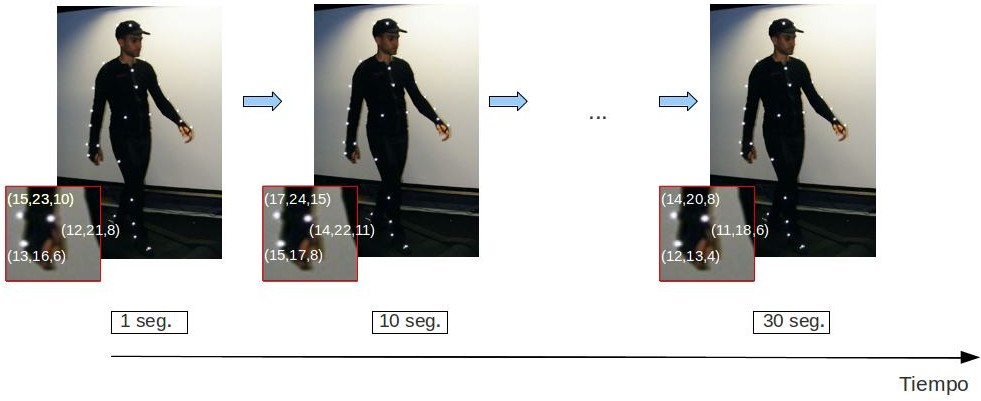
\includegraphics[scale=0.4]{img/Sistema_completo/diagrama_abuelas_2.jpg}
\end{center}
\caption{Posición de los marcadores a lo largo del tiempo.}
\label{abuela2}
\end{figure}

Dicho de otra forma, la aplicación a desarrollar recibe como entrada imágenes de video desde varias cámaras capturando el movimiento de una persona desde distintos ángulos. Dichas cámaras deben estar previamente calibradas. A partir de las imágenes obtenidas se detectan distintos puntos de referencia del cuerpo según el estudio particular que se desee realizar. Este proceso se realiza para cada imagen del video obteniendo así la trayectoria en tres dimensiones de cada punto a lo largo del tiempo. Luego, a partir del procesamiento de la posición 3D de los puntos se obtendrán otros datos estadísticos de interés para el usuario.

\begin{figure}[H]
\begin{center}
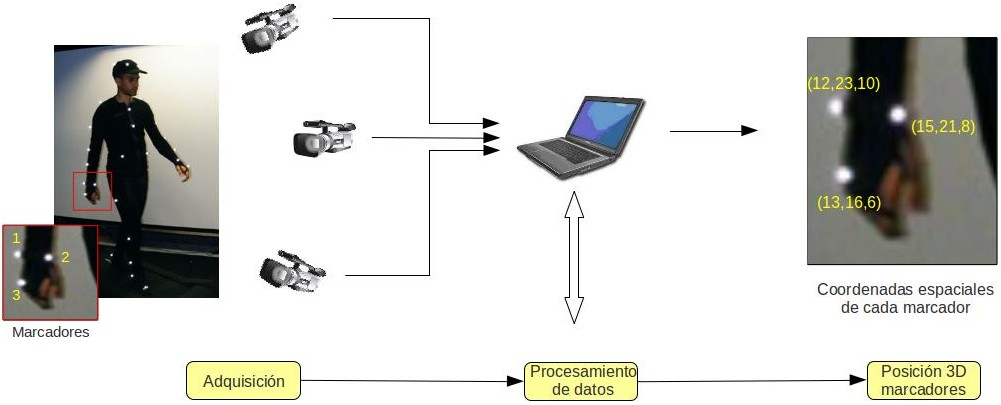
\includegraphics[scale=0.4]{img/Sistema_completo/diagrama_abuelas_1.jpg}
\end{center}
\caption{Funcionamiento de un sistema de captura de movimiento.}
\label{abuela1}
\end{figure}

\vspace{5 mm}

%SINOPSIS
El proyecto comenzó con una profunda investigación y revisión bibliográfica, en particular se buscaron diseños de sistemas de captura de movimiento ya estudiados y detalles de implementación de cada bloque en conjunto o individuales. 

Además, se hizo incapié en obtener una base de datos con secuencias (ya sean reales o sintéticas) para probar la implementación. Esta búsqueda en particular no obtuvo buenos resultados, ya que no se encontraron bases de datos acordes a lo necesitado. Por esto, se decidió implementar una base de datos propia.

 Luego se definió la metodología a implementar. De acuerdo a la bibliografía consultada, se optó por un sistema de 4 bloques principales cómo se muestra en la figura \ref{bloquesSistintro}. 

 \begin{figure}[H]
\begin{center}
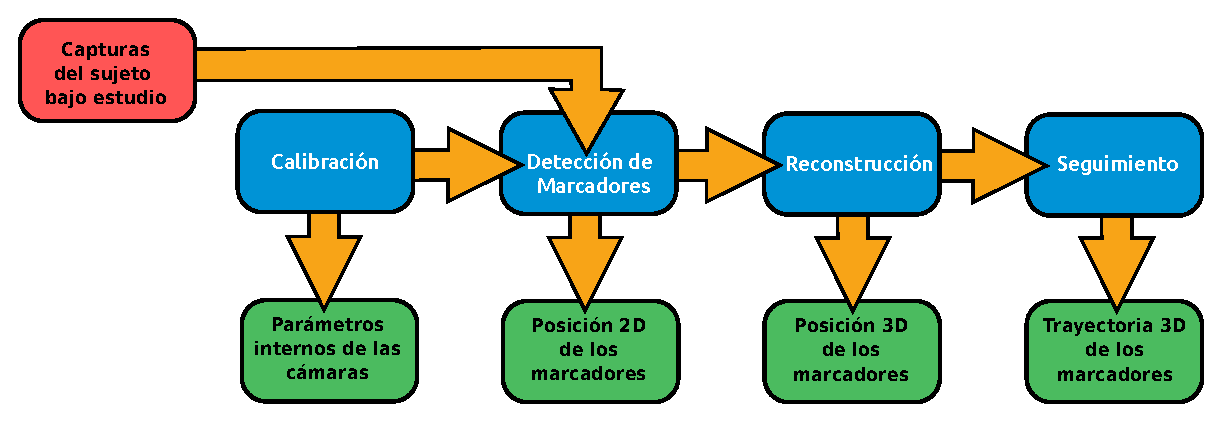
\includegraphics[scale=0.8]{img/Sistema_completo/Diagrama_de_bloques.eps}
\end{center}
\caption{Diagrama de bloques del sistema a implementar.}
\label{bloquesSistintro}
\end{figure}

Cada uno de estos bloques realiza una actividad bien definida:
\begin{itemize}
\item El bloque de \emph{calibración}, es el encargado de realizar la sincronización de las múltiples cámaras utilizadas para realizar la captura y obtener los parámetros internos de las mismas, para saber la posición que tiene cada una en el espacio y de esta manera realizar una correcta reconstrucción de los puntos.
\item El bloque \emph{detección de marcadores}, es el encargado de identificar cada marcador en las imagenes obteniendo la posición 2D de cada uno de ellos a lo largo de la secuencia de captura y para cada cámara (ver figura \ref{peladocirculosintrointro}).
\item Con los datos de la posición 2D de los marcadores desde distintas vistas, se obtiene la posición 3D de cada uno a través del bloque \emph{reconstrucción} (ver figura \ref{peladoewconstruidointro}).
\item Por último, se relaciona cada marcador en un cuadro de la secuencia con su correspondiente en el resto de los cuadros, obteniendo asi la trayectoria de cada punto a lo largo del tiempo. Esto se realiza en el bloque \emph{seguimiento} (ver figura \ref{peladoetrackingintro}).
\end{itemize}

Cabe destacar que estos bloques se implementaron independientemente unos de otros, de esta forma se pueden realizar modifcaciones en uno de ellos sin afectar el funcionamiento de los otros. Este aspecto toma gran relevancia en etapas futuras, si se necesita optimizar alguno de estos bloques en particular, o agrear alguna característica para procesar datos de algun caso de uso determinado. De no presentar esta particularidad, la modificación de un bloque podría afectar negativamente el funcionamiento del sistema entero.

\begin{figure}[H]
        \centering
        \subfloat[Captura original]{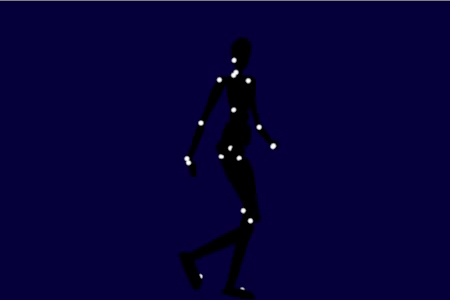
\includegraphics[scale=0.4]{img/peladoFondoAzul.png}\label{peladoOriginalintrointro}}\hspace{3 mm}
        \subfloat[Detección de marcadores]{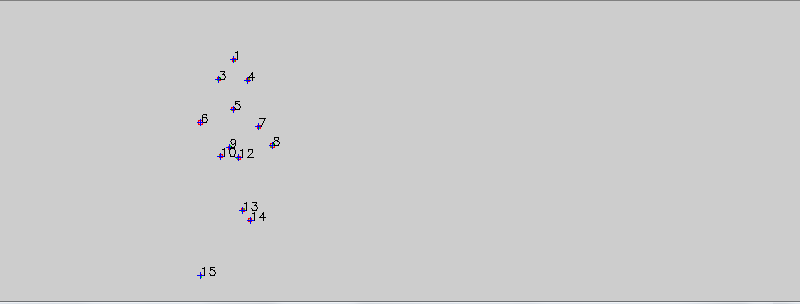
\includegraphics[scale=0.4]{img/peladoFondoAzul_circulos.png}\label{peladocirculosintrointro}}

        \subfloat[Recontrucción 3D]{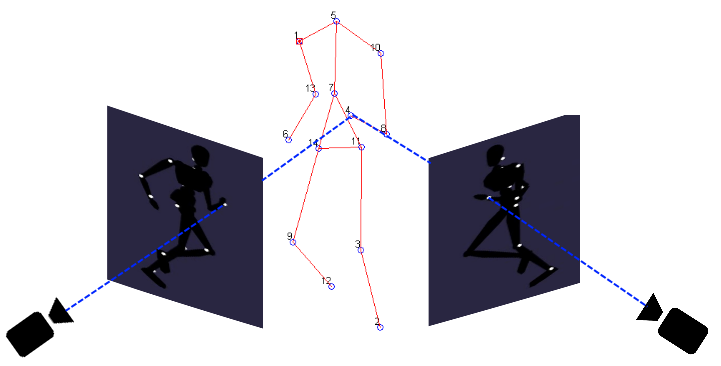
\includegraphics[scale=0.3]{img/Reconstruccion/reconstruccion2.png}\label{peladoewconstruidointro}}
    	\subfloat[Seguimiento]{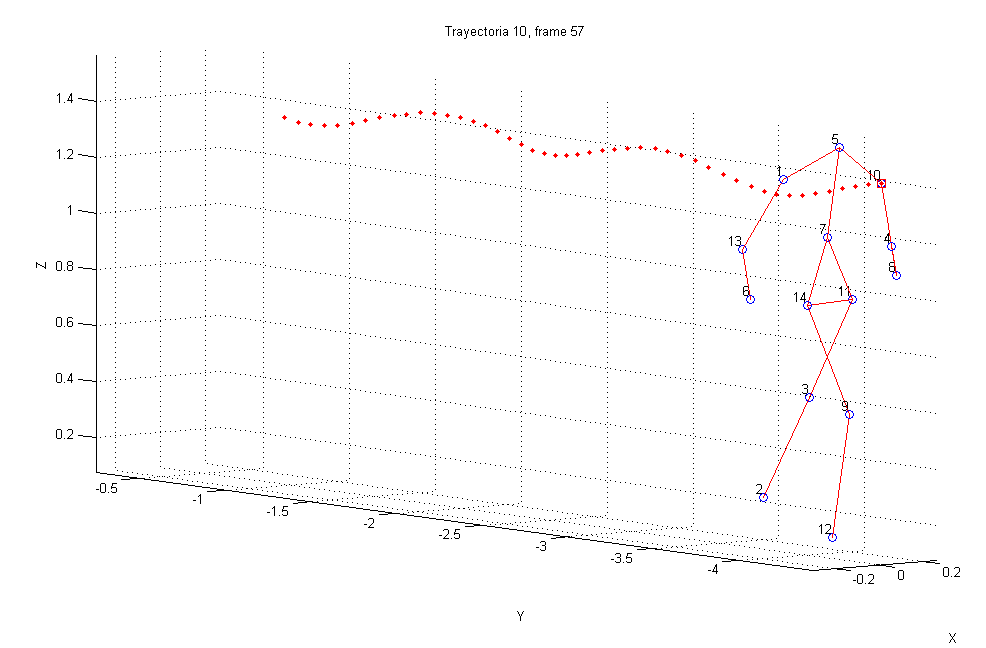
\includegraphics[scale=0.3]{img/Tracking/track1.png}\label{peladoetrackingintro}}  
  \caption{Salidas de los bloques principales del sistema.}
      \label{ejemplotutiintro}
\end{figure}

A continuación, se presenta una breve revisión del estado del arte de los sistemas de captura de movimiento. Luego, la documentación continúa con la explicación de la base de datos generada y la justificación e implementación de cada bloque del sistema mencionado anteriormente. Finalmente se realiza un análisis de los resultados obtenidos y de la performance del sistema en general.

\subsection{Estado del arte}
%%%%%%%%%%%%%%%%%%%%%%%%%%%%%%%%%%%%%%%%%%%%%%%%%%%%%%%%%%%%%%%%%%%%%%%%%%%%%%%%%%%%%%%%%%%%%%%%%%%%%%%%%%%%%%%%%%%%%%%%%%%%%%%%%%%5
%qué opciones tengo para hacerlo? por qué hay estas opciones? para qué se usan?
%%%%%%%%%%%%%%%%%%%%%%%%%%%%%%%%%%%%%%%%%%%%%%%%%%%%%%%%%%%%%%%%%%%%%%%%%%%%%%%%%%%%%%%%%%%%%%%%%%%%%%%%%%%%%%%%%%%%%%%%%%%%%%%%%%%

Al día de hoy existen varios sistemas de captura de movimiento, desafortunadamente los más completos son sistemas bajo costo de licenciamiento. 

Como se mencionó anteriormente, los más populares actualmente son los que se utilizan en la industria del cine o de diseño de videojuegos. En este contexto, se almacenan las acciones de actores humanos y se usa esta información para animar modelos digitales de personajes en animación 3D.

Algunos ejemplos de sistemas de captura de movimiento bajo licencia son:

\begin{itemize}
\item \emph{Vicon}\footnote{http://www.vicon.com/}. Es una empresa que vende sistemas de captura de movimiento, tanto software como hardware. Sus sistemas son muy conocidos y de los más utilizados para estudios clínicos y biomecánicos en el mundo, asi cómo para otras investigaciones científicas. En particular, este sistema está siendo utilizado en el Departamento de Fisiatría y Rehabilitación del Hospital de Clínicas. Presenta como ventajas frente a otros sistemas la velocidad con que realiza el procesamiento de los datos y la calidad de las cámaras para realizar las capturas.
\item \emph{Qualisys}\footnote{http://www.qualisys.com/} Junto con Vicon son los dos sistemas de captura de movimiento más utilizados en el ámbito de la investigación científica. Presenta como ventajas frente al anterior la utilización del modelo AIM\footnote{Automatic Identification of Markers}, que básicamente es un identificador de marcadores que ``aprende'' de cada secuencia procesada ahorrando mucho tiempo y trabajo en identificar marcadores. Además presenta una interfaz de usuario más amigable y requiere menos tiempo en aprender a utilizar.
\item \emph{OptiTrack}\footnote{http://www.naturalpoint.com/optitrack/}. Es de los sistemas comerciales más baratos, cerca de la cuarta parte de lo que cuesta un sistema Vicon por ejemplo. Además, otra de sus ventajas es que brinda acceso a bajo nivel a través de un conjunto de  SDK's y API's tanto para el hardware como para los datos que obtiene, permitiendo manipular los mismos y procesarlos de la manera que se desee por fuera de las aplicaciones que provee. 
\item \emph{Massive}\footnote{http://www.massivesoftware.com/}. Es un software destinado a producir efectos especiales para cinematografía, programas televisivos y videojuegos entre otras cosas. El software cuenta con varios productos para producir distintos tipos de efectos y animaciones, entre ellos la caputra de movimiento. Fue originalmente diseñado par utilizar en la trilogía de El Señor De Los Anillos de Peter Jackson y desde entonces se ha convertido en uno de los mejores software para realizar efectos visuales de muchedumbres y animación de personajes autónomos.
\item \emph{Motion Analysis}\footnote{http://www.motionanalysis.com/}.
\item \emph{PhaseSpace}\footnote{http://www.phasespace.com/}.
\end{itemize}

Los sistemas anteriores, y la mayoría de los sistemas de captura de movimiento modernos, utilizan como marcadores sensores infrarrojos o leds. Estos últimos facilitan de gran forma la etapa de detección de marcadores en cada cámara, mientras que para el caso de los sensores infrarrojos no se tiene una etapa de detección ya que los mismos envían la información de la posición directamente.

La gran desventaje de los sistemas anteriores es su costo monetario. A modo de ejemplo, un sistema Vicon de 10 cámaras cuesta aproximadamente \$70.000 USD\footnote{Este precio depende fuertemente del tipo de cámara que se utilice, los precios de las mismas no bajan de los \$3.000 USD por unidad.}.

Por otro lado, también existen softwares de captura de movimiento Open Source, como por ejemplo Kinovea\footnote{http://www.kinovea.org/}. Está enfocado al deporte, permitiendo analizar y mejorar la técnica de los atletas a través del procesamiento de secuencias de video. Permite, entre otras cosas, medir distancias, ángulos y tiempos manualmente o utilzar un tracking semi-automático para seguir puntos en vivo y obtener su trayectoria. La gran desventaja que presenta frente a otros sistemas es que realiza unicamente análisis en 2D.

%Dada las características de este proyecto otro antecedente relevante a tener en cuenta en el área, es el de un grupo de investigadores del Hospital de Clínicas que junto al grupo de Tratamiento de Imágenes de la Facultad de Ingeniería han estudiado previamente la marcha de las personas a los efectos de reconocer en ellas patrones de movimiento. Dicho proyecto recibe el nombre “Cíclope”.